\documentclass[12pt,reqno,final]{amsart}\usepackage[]{graphicx}\usepackage[]{color}
%% maxwidth is the original width if it is less than linewidth
%% otherwise use linewidth (to make sure the graphics do not exceed the margin)
\makeatletter
\def\maxwidth{ %
  \ifdim\Gin@nat@width>\linewidth
    \linewidth
  \else
    \Gin@nat@width
  \fi
}
\makeatother

\definecolor{fgcolor}{rgb}{0.345, 0.345, 0.345}
\newcommand{\hlnum}[1]{\textcolor[rgb]{0.686,0.059,0.569}{#1}}%
\newcommand{\hlstr}[1]{\textcolor[rgb]{0.192,0.494,0.8}{#1}}%
\newcommand{\hlcom}[1]{\textcolor[rgb]{0.678,0.584,0.686}{\textit{#1}}}%
\newcommand{\hlopt}[1]{\textcolor[rgb]{0,0,0}{#1}}%
\newcommand{\hlstd}[1]{\textcolor[rgb]{0.345,0.345,0.345}{#1}}%
\newcommand{\hlkwa}[1]{\textcolor[rgb]{0.161,0.373,0.58}{\textbf{#1}}}%
\newcommand{\hlkwb}[1]{\textcolor[rgb]{0.69,0.353,0.396}{#1}}%
\newcommand{\hlkwc}[1]{\textcolor[rgb]{0.333,0.667,0.333}{#1}}%
\newcommand{\hlkwd}[1]{\textcolor[rgb]{0.737,0.353,0.396}{\textbf{#1}}}%
\let\hlipl\hlkwb

\usepackage{framed}
\makeatletter
\newenvironment{kframe}{%
 \def\at@end@of@kframe{}%
 \ifinner\ifhmode%
  \def\at@end@of@kframe{\end{minipage}}%
  \begin{minipage}{\columnwidth}%
 \fi\fi%
 \def\FrameCommand##1{\hskip\@totalleftmargin \hskip-\fboxsep
 \colorbox{shadecolor}{##1}\hskip-\fboxsep
     % There is no \\@totalrightmargin, so:
     \hskip-\linewidth \hskip-\@totalleftmargin \hskip\columnwidth}%
 \MakeFramed {\advance\hsize-\width
   \@totalleftmargin\z@ \linewidth\hsize
   \@setminipage}}%
 {\par\unskip\endMakeFramed%
 \at@end@of@kframe}
\makeatother

\definecolor{shadecolor}{rgb}{.97, .97, .97}
\definecolor{messagecolor}{rgb}{0, 0, 0}
\definecolor{warningcolor}{rgb}{1, 0, 1}
\definecolor{errorcolor}{rgb}{1, 0, 0}
\newenvironment{knitrout}{}{} % an empty environment to be redefined in TeX

\usepackage{alltt}
\usepackage[round,numbers,sort&compress]{natbib}
\usepackage{graphicx}
\usepackage{times}
\usepackage{rotating}
\usepackage{subfig}

\title[]{}

\setlength{\textwidth}{6.25in}
\setlength{\textheight}{8.75in}
\setlength{\evensidemargin}{0in}
\setlength{\oddsidemargin}{0in}
\setlength{\topmargin}{-.35in}
\setlength{\parskip}{.1in}
\setlength{\parindent}{0.0in}

\theoremstyle{plain}
\newtheorem{thm}{Theorem}
\newtheorem{corol}[thm]{Corollary}
\newtheorem{prop}[thm]{Proposition}
\newtheorem{lemma}[thm]{Lemma}
\newtheorem{defn}[thm]{Definition}
\newtheorem{hyp}[thm]{Hypothesis}
\newtheorem{example}[thm]{Example}
\newtheorem{conj}[thm]{Conjecture}
\newtheorem{algorithm}[thm]{Algorithm}
\newtheorem{remark}{Remark}
\renewcommand\thethm{\arabic{thm}}
\renewcommand{\theremark}{}

\numberwithin{equation}{part}
\renewcommand\theequation{\arabic{equation}}
\renewcommand\thesection{\arabic{section}}
\renewcommand\thesubsection{\thesection.\arabic{subsection}}
\renewcommand\thefigure{\arabic{figure}}
\renewcommand\thetable{\arabic{table}}
\renewcommand\thefootnote{\arabic{footnote}}
\IfFileExists{upquote.sty}{\usepackage{upquote}}{}
\begin{document}

\maketitle

This documents my exploration of the differences between \texttt{OUwie} and \texttt{ouch} when each is asked to fit OU models with a single $\alpha$ and $\sigma$ operating on the entire tree.
The motivation for this is that I noticed that the parameter estimates and likelihoods reached by \texttt{OUwie} and \texttt{ouch} are often quite different.
I originally did this is 2014, but wanted to update it now to explore how the programs differ from one another now.
You can see the results from 2014 in this document as well (Figs. 4-6).

The procedure I will follow here is very straightforward: generate Yule trees of different sizes; specify two selective regimes arising out of the branching event at the root, so that there is a single monophyletic clade in each selective regime - this is the simplest possible multiple-optimum OU scenario; simulate phenotypic data with a known $\alpha$ and $\sigma$; fit an OU model to the phenotypic data and tree using both \texttt{OUwie} and \texttt{ouch} and record the parameter estimates and likelihoods.

Trees were generated by assuming that branching follows a Poisson process, so that branching events are exponentially distributed. To generate trees of different sizes, I set the rate parameter of the exponential distribution to a value of 0.3 and found random number generator seeds that would generate trees of size from 10 to 100 tips, with the only constraint being that the smaller of the two clades originating at the root had at least 1/3 of the total tip species.
This guarantees that both selective regimes are reasonably well-represented, thereby improving both power and parameter estimates.

Phenotypic data was generated assuming $\alpha=3$ and $\sigma^2=1$, with selective optima of $\theta_1=-1$ and $\theta_2=1$. The root was always assumed to be in regime 1. For any given tree size, 20 different phenotypic datasets were generated and fit to the OU model.
This allows me to calculate how bias/variance in parameter estimates differ between the two algorithms.
All of the code, including random number generator seeds, needed to reproduce the results shown here can be found in this file.

\begin{knitrout}
\definecolor{shadecolor}{rgb}{0.969, 0.969, 0.969}\color{fgcolor}\begin{kframe}


{\ttfamily\noindent\itshape\color{messagecolor}{\#\# `geom\_smooth()` using method = 'gam' and formula 'y \textasciitilde{} s(x, bs = "{}cs"{})'}}\end{kframe}\begin{figure}
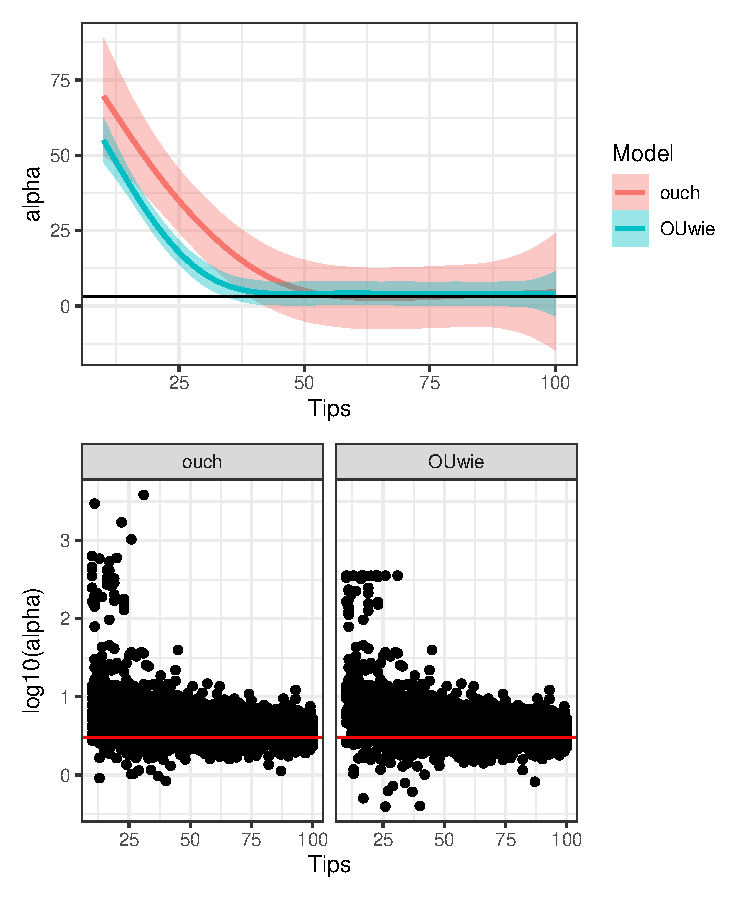
\includegraphics[width=\maxwidth]{figure/unnamed-chunk-1-1} \caption[Comparing the $\alpha$ estimates of \texttt{ouch} and \texttt{OUwie} for trees of 10-100 tips]{Comparing the $\alpha$ estimates of \texttt{ouch} and \texttt{OUwie} for trees of 10-100 tips. In the top panel, the lines and shaded region come from fitting a generalized additive model to the $\alpha$ estimates, with the size of the tree as the dependent variable. The line shows the expectation of the GAM, whereas the shaded regions capture the variability across the 20 stochastically generated phenotypic datasets. From this figure, it is clear that both methods converge on very similar estimates, with very similar error, as the two sit essentially right on top of one another. A closer examination of the estimates for each dataset (bottom panels) shows that variability is still fairly large.}\label{fig:unnamed-chunk-1}
\end{figure}


\end{knitrout}

\begin{knitrout}
\definecolor{shadecolor}{rgb}{0.969, 0.969, 0.969}\color{fgcolor}\begin{kframe}


{\ttfamily\noindent\itshape\color{messagecolor}{\#\# `geom\_smooth()` using method = 'gam' and formula 'y \textasciitilde{} s(x, bs = "{}cs"{})'}}\end{kframe}\begin{figure}
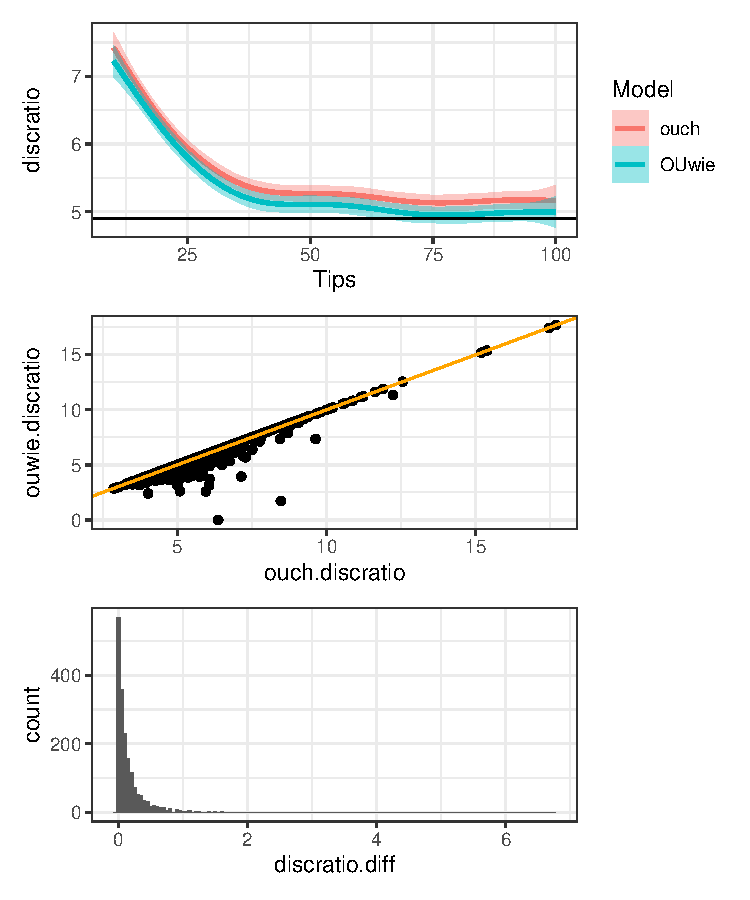
\includegraphics[width=\maxwidth]{figure/unnamed-chunk-2-1} \caption{Estimates of the discriminability ratio, $\sqrt{2\alpha}\Delta\theta/\sigma$ (Cressler, Butler, and King 2015). This dimensionless combination of parameters may be better estimated than any individual parameter. This dimensionless parameter also captures the linked ability to estimate the selective optima, selection strength, and drift. You can see from all three panels that \texttt{ouch} and \texttt{OUwie} often estimate this parameter nearly identically: the top panel shows results from a generalized additive model fit to the estimates for each number of tips; the middle panel shows a scatterplot of the estimates for each method; the bottom panel shows a histogram of the difference between the \texttt{ouch} estimate and the \texttt{OUwie} estimate. Interestingly, the estimate returned by \texttt{ouch} is always larger than the estimate returned by \texttt{OUwie}, which is why \texttt{OUwie} tends to do a better job estimating the parameter.}\label{fig:unnamed-chunk-2}
\end{figure}


\end{knitrout}

\begin{knitrout}
\definecolor{shadecolor}{rgb}{0.969, 0.969, 0.969}\color{fgcolor}\begin{figure}
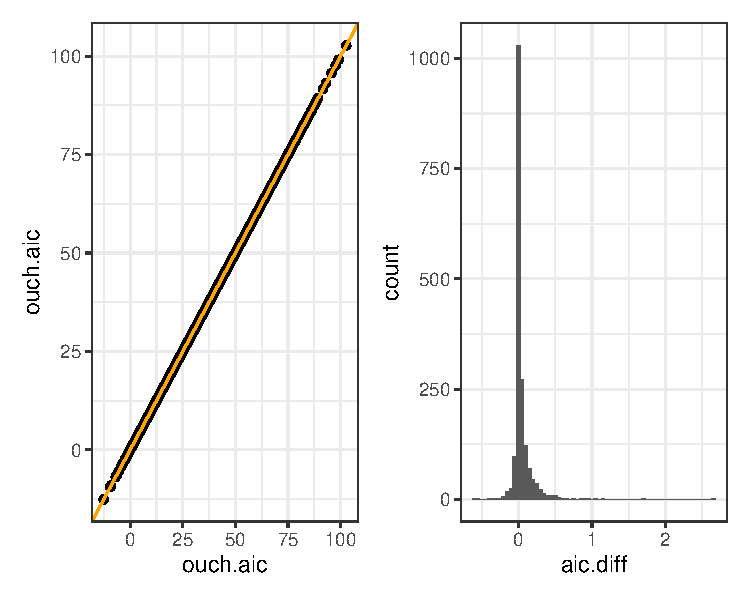
\includegraphics[width=\maxwidth]{figure/unnamed-chunk-3-1} \caption{Estimated AICs for \texttt{ouch} and \texttt{OUwie} are essentially identical. The histogram shows the difference between the AIC of the parameters estimated by \texttt{ouch} and the AIC of the \texttt{OUwie} parameter estimates; positive values suggest that \texttt{OUwie} has found parameter estimates with a higher likelihood.}\label{fig:unnamed-chunk-3}
\end{figure}


\end{knitrout}

\newpage

Fig. 4-6 shows all of the results from 2014.
A key point is that all of the trees, regimes, and phenotypic datasets used in 2014 are \emph{identical} to the trees, regimes, and phenotypic datasets used in 2020.
The only difference in fits is due to difference in either \texttt{ouch} or \texttt{OUwie}: I assume it's mostly due to changes in \texttt{OUwie}, rather than \texttt{ouch}, since \texttt{OUwie} is under more active maintenance and updating.

\begin{knitrout}
\definecolor{shadecolor}{rgb}{0.969, 0.969, 0.969}\color{fgcolor}\begin{kframe}


{\ttfamily\noindent\itshape\color{messagecolor}{\#\# `geom\_smooth()` using method = 'gam' and formula 'y \textasciitilde{} s(x, bs = "{}cs"{})'}}\end{kframe}\begin{figure}
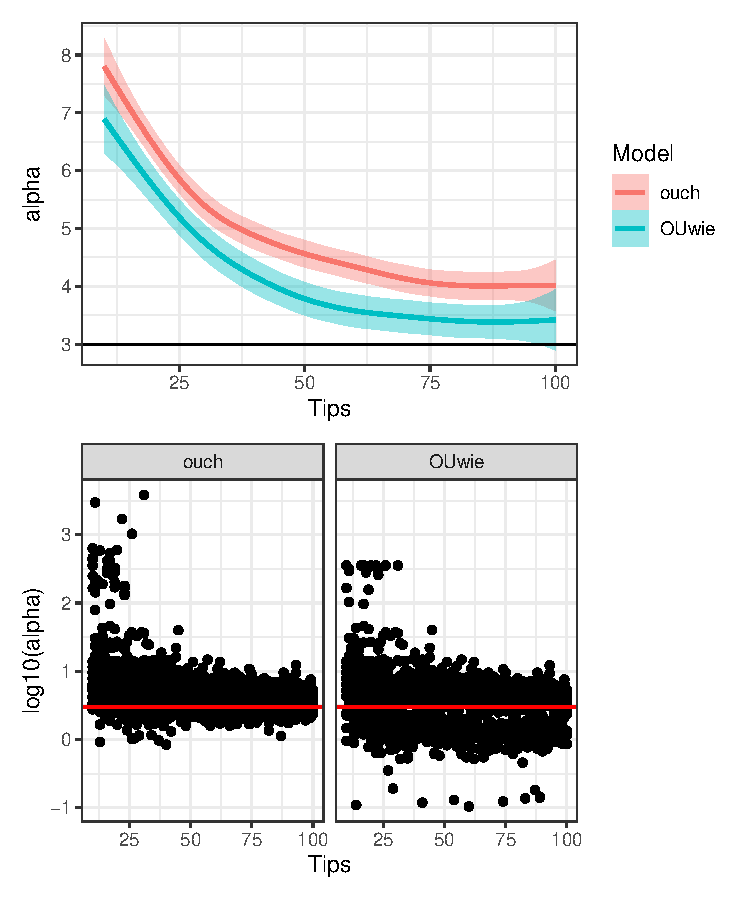
\includegraphics[width=\maxwidth]{figure/unnamed-chunk-4-1} \caption{Comparing the $\alpha$ estimates of \texttt{ouch} and \texttt{OUwie} for trees of 10-100 tips, using the 2014 version of \texttt{OUwie}. Despite what the GAM is showing in the top panel, it's clear from the bottom panel that there is less variability for large trees in \texttt{ouch}.}\label{fig:unnamed-chunk-4}
\end{figure}


\end{knitrout}

\begin{knitrout}
\definecolor{shadecolor}{rgb}{0.969, 0.969, 0.969}\color{fgcolor}\begin{kframe}


{\ttfamily\noindent\itshape\color{messagecolor}{\#\# `geom\_smooth()` using method = 'gam' and formula 'y \textasciitilde{} s(x, bs = "{}cs"{})'}}\end{kframe}\begin{figure}
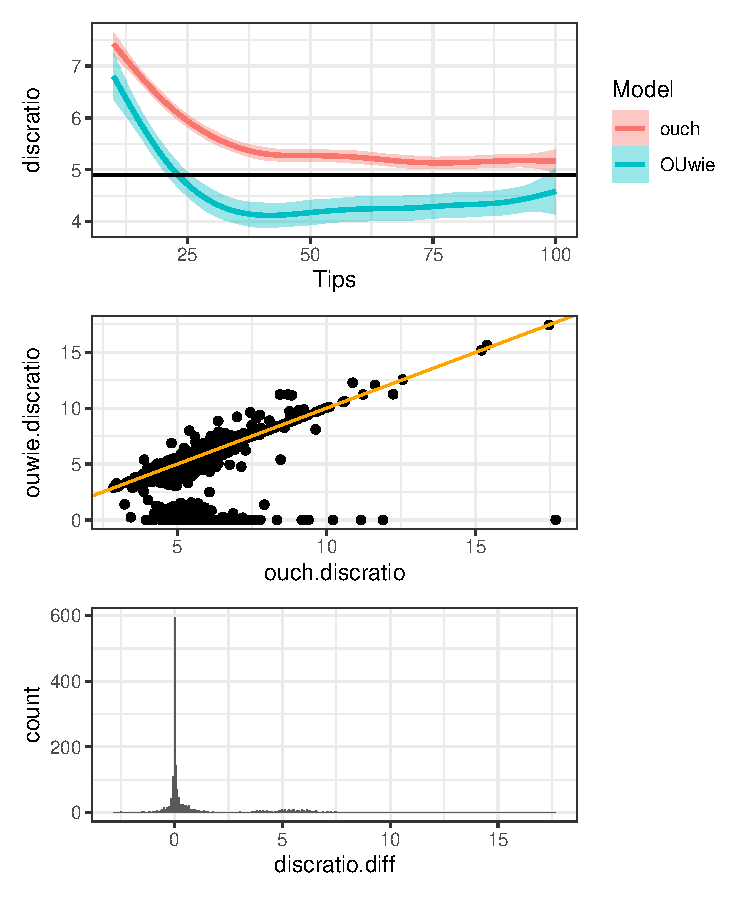
\includegraphics[width=\maxwidth]{figure/unnamed-chunk-5-1} \caption{Estimates of the discriminability ratio, $\sqrt{2\alpha}\Delta\theta/\sigma$ (Cressler, Butler, and King 2015). It is clear that this is better estimated by \texttt{ouch} than it is by the 2014 version of \texttt{OUwie}.}\label{fig:unnamed-chunk-5}
\end{figure}


\end{knitrout}

\begin{knitrout}
\definecolor{shadecolor}{rgb}{0.969, 0.969, 0.969}\color{fgcolor}\begin{figure}
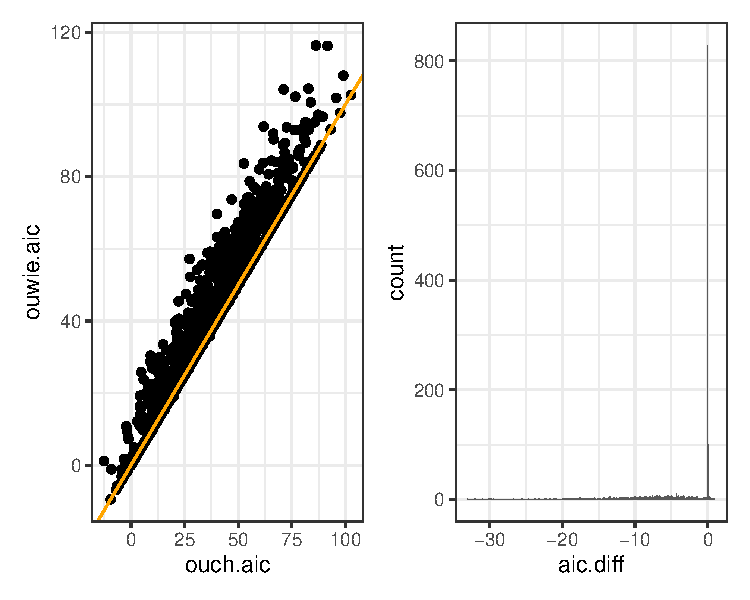
\includegraphics[width=\maxwidth]{figure/unnamed-chunk-6-1} \caption[Estimated AICs for \texttt{ouch} and the 2014 version of \texttt{OUwie} show that \texttt{ouch} tends to find parameter estimates with a lower AIC (because the difference between the \texttt{ouch} AIC and the \texttt{OUwie} AIC is typically negative]{Estimated AICs for \texttt{ouch} and the 2014 version of \texttt{OUwie} show that \texttt{ouch} tends to find parameter estimates with a lower AIC (because the difference between the \texttt{ouch} AIC and the \texttt{OUwie} AIC is typically negative.}\label{fig:unnamed-chunk-6}
\end{figure}


\end{knitrout}

\newpage


\end{document}
